




\section{BeagleBone Black User guide}
\noindent The most common way to interact with the BeagleBone Black (BBB) is by connecting to a terminal on it via a host computer. The software needed to do it differ depending on the operating system of the host. 


\subsection{Linux host}
\noindent The Linux terminal can connect to a terminal in a BBB via Ethernet via the ssh command. SSH is included in most Linux distributions by default.
\begin{lstlisting}[language=bash]
  $ ssh ubuntu@192.168.1.1 
\end{lstlisting}
\noindent On this line, ubuntu is the user name and 192.168.1.1 is the IP of the BBB. A prompt will ask for a password, the password is ubuntu.


\subsection{Windows host}


\begin{figure}[!ht]
	\begin{center}
		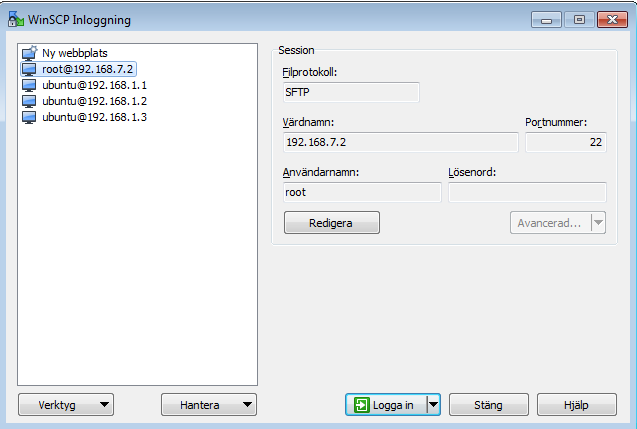
\includegraphics[width=80mm]{./Images/Software/WinSCP.png}
		\caption{WinSCP}
		\label{WinSCP}
	\end{center}
\end{figure}

\noindent WinSCP\cite{WinSCP}, Secure Copy (SCP), is an application for managing files between Windows and BBB easier. One can move files freely between the both systems without terminal commands.
If connected through Ethernet over the switch use hostname ("värdnamn" in fig. \ref{WinSCP}) 192.168.1.n where n is dependent on which of the BBB one wants to access.
If connected through USB use hostname 192.168.7.2. With drivers, this can also share connection to internet for installation of applications etc in BBB.
Username ("Användarnamn" in fig. \ref{WinSCP}) is either root or ubuntu. If ubuntu then password is ubuntu.

\begin{figure}[!ht]
	\begin{center}
		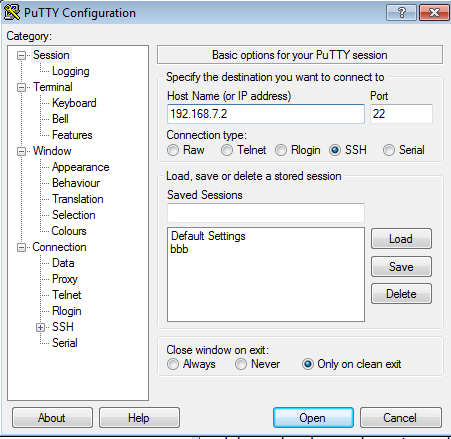
\includegraphics[width=80mm]{./Images/Software/Putty.png}
		\caption{PuTTY}
		\label{YourLabel}
	\end{center}
\end{figure}

PuTTY \cite{PuTTY} is an application to Secure Shell (SSH) in to BBB from Windows. This gives the possibility to remote control the BBB. By doing this one can compile and run applications.

\subsection{A Linux environment}

\noindent When connected, the user has to navigate in the Linux environment on BBB. This is not effected by the operating system of the host. Navigation in Linux is mostly done with two commands:
\begin{lstlisting}[language=bash]
  $ ls 
\end{lstlisting}
\noindent This command ls show all the folders in the current directory.
\begin{lstlisting}[language=bash]
  $ cd Software/
\end{lstlisting}
\noindent The cd command is used to enter a folder.
\begin{lstlisting}[language=bash]
  $ cd ..
\end{lstlisting}
\noindent The folder name .. will move up one level. Note that Linux is case sensitive regarding names.

All of the software is located in the folder /home/ubuntu/BBB/software/. All the binary files should be located in a folder called 'bin' within the folder Software. To transfer files or folders between a computer and a BBB, use the following command:
\begin{lstlisting}[language=bash]
  $ scp -r pid/ ubuntu@192.168.1.1:BBB/software/
\end{lstlisting}
\noindent The flag -r tells the program that the source 'pid/' is a folder while ubuntu@192.168.1.1 is the user on the target computer, in this case a BBB. The colon is the separator where the path target path begin. The default folder will be /home/ubuntu. By adding BBB/software/, the folder will end up at /home/ubuntu/BBB/software/pid with all its content.

\noindent If gcc is installed, a project can be compiled with gnatmake.
\begin{lstlisting}[language=bash]
  $ gnatmake -P mainproject.gpr
\end{lstlisting}
\noindent Or to only compile a single file:
\begin{lstlisting}[language=bash]
  $ gnatmake main.adb
\end{lstlisting}

\noindent To make the process easier, a makefile can be used. Here is an example with three commands. Note that the formatting is important.
\begin{lstlisting}[language=bash]
this:
	gnatmake -P mainproject.gpr
all:
	gnat clean -r -P mainproject.gpr
	gnatmake -P mainproject.gpr
clean:
	gnat clean -r -P mainproject.gpr
\end{lstlisting}

\noindent The command make will run the first command in the makefile, 'this'. With other words, the project mainproject.gpr will be compiled. To run another command, add the name after make.
\begin{lstlisting}[language=bash]
  $ make all
\end{lstlisting}

\noindent This will clean the project and rebuild it from scratch. Multiple makefiles can be combined with a shell script so all of them can be compiled by just running the shell script. 
\begin{lstlisting}[language=bash]
  $ make all -C software/myprojectfolder/
\end{lstlisting}
\noindent This command will run a makefile located in the folder software/myprojectfolder/, multiple lines can be added to compile mulitple projects. To run an executable file, use ./ before the name.
\begin{lstlisting}[language=bash]
  $ ./main
\end{lstlisting}
\noindent To exit a program, press ctrl + c. To check which processes are running use ps aux.
\begin{lstlisting}[language=bash]
  $ ps aux
\end{lstlisting}
\noindent There are currently a script file with some predefined functions. The file system.sh is a shell script located at /home/ubuntu/BBB/. It can make some tasks easier. It got 5 commands, kill, run, build, restart and move. The command kill together with a name will end that process.
\begin{lstlisting}[language=bash]
  $ ./system.sh kill pid
\end{lstlisting}
\noindent This will end the PID controller. To kill all the running nodes, leave leave the name empty. All of the commands except build can be used this way. With other words, the run command will look like this.
\begin{lstlisting}[language=bash]
  $ ./system.sh run pid
\end{lstlisting}
\noindent The run command will start the node as a background process but it will still output all the messages to the terminal. To hide the output, redirect the standard output with a pipe to null.
\begin{lstlisting}[language=bash]
  $ ./system.sh run pid > /dev/null
\end{lstlisting}
\noindent The build command will compile all projects. If the parameter all is added, all projects will be cleaned first. The build command does also move all the executable files to a specific binary folder. This folder is used by run and restart. The restart command simply kills a specified process and tries to run it again. Finally, the command move will only copy the executable file(s) to the binary folder.

\subsection{BeagleBone Black configurations}
To setup a new BeagleBone Black card (BBB) some configurations has to be done.

First, to install the Bone Debian operating system on the BBB simply download the latest release of Bone Debian operating system for the BBB at \url{http://beagleboard.org/latest-images} and mount it to a microSD card using any mounting software. One can either choose the eMMC version which installs the operating system onto the internal flash memory on the BBB or the version which runs directly from the microSD card which does not require any flashing of the internal memory.

Once the operating system has been installed onto the BBB some further configurations has to be done.
To configure the Ethernet network communication on the BBB run the following command where the X should be a number between 2 and 254 that makes the BBB unique on the network.
\begin{lstlisting}[language=bash]
  $ ifconfig 192.168.1.X netmask 255.255.255.0
\end{lstlisting}

UART communication is allowed by echoing the desired UART ports to the BBB cape that is installed with the operating system.
\begin{lstlisting}[language=bash]
	$ echo BB-UART1 > /sys/devices/bone_capemgr.*/slots
	$ echo BB-UART4 > /sys/devices/bone_capemgr.*/slots
\end{lstlisting}

Some of the commands could preferably be put into a boot up script since it sometimes stores the new configurations temporary.

